\documentclass[11pt]{book}
\usepackage{gvv-book}
\usepackage{gvv}
\usepackage[sectionbib,authoryear]{natbib}
\setcounter{secnumdepth}{3}
\setcounter{tocdepth}{2}
\makeindex
\begin{document}
\frontmatter
\tableofcontents
\setcounter{page}{1}
\mainmatter
\chapter{Triangle}
Consider a triangle with vertices
\begin{align}
\label{eq:tri-pts}
\vec{A}=\myvec{5 \\ -2},\,
\vec{B}=\myvec{-5\\5},\,
	\vec{c}=\myvec{-2\\-5},\,
\end{align}
\section{Vectors}
\begin{enumerate}[label=\thesection.\arabic*.,ref=\thesection.\theenumi]
\numberwithin{equation}{enumi}

\item The direction vector of $AB$ is defined as
		\begin{align}
			\vec{B}-
			\vec{A}
		\end{align}
Consider a triangle with vertices
\begin{align} 
 \vec{A} &= \myvec{ 5\\ -2 } \\ \vec{B} &= \myvec{ -5\\ 5 }
  \\\vec{C} &= \myvec{ -2\\ -5}
 \end{align}
The Direction Vector of $AB$ is defined as 
\begin{align} 
\vec{B} - \vec{A}
\end{align}
Question1.1.1 :Find the Direction Vectors of $AB$,$BC$,$CA$.\\
\solution

\begin{enumerate} 
\item  The Direction vector of $AB$ is \begin{align} &= \vec{B} - \vec{A} \\
 &= \myvec{-5 - (5)\\ 5 - (-2) } \\&= \myvec{ -10\\ 7 }
 \end{align}
 
\item The Direction vector of $BC$ \begin{align}&= \vec{C} - \vec{B}\\
 &= \myvec{ -2 - (-5)\\ -5 - 5 } \\&= \myvec{3\\ -10 }
  \end{align}
  
  \item  The Direction vector of $CA$  \begin{align} &= \vec{A} - \vec{C} \\ 
 &= \myvec{ 5 - (-2)\\ -2 - (-5) } \\&= \myvec{ 7\\ 3 }
  \end{align}
 \end{enumerate}

\item The length of side $BC$ is 
		\begin{align}
			\norm{\vec{B}-\vec{A}} \triangleq \sqrt{\brak{\vec{B}-\vec{A}}^{\top}{\vec{B}-\vec{A}}}
		\end{align}
		where
		\begin{align}
			\vec{A}^{\top}\triangleq\myvec{1 & 0}
		\end{align}
Question 1.1.2 : Find the length of side AB, BC, CA.\\
\solution
Solving for AB
Given, 
\begin{align}
\vec{A} = \myvec{5\\-2},
\vec{B} = \myvec{-5\\5},
\vec{C} = \myvec{-2\\-5} \\  
 \norm{\vec{B}-\vec{A}}\ &=  \sqrt{\brak{\vec{B}-\vec{A}}^{\top}\brak{\vec{B}-\vec{A}}} \\
 \vec{B}-\vec{A} &= \myvec{-5\\ 5} - \myvec{5 \\ -2} \\
 \vec{B}-\vec{A} &= \myvec{-10\\ 7} \\
 \brak{\vec{B}-\vec{A}}^{\top} &= {\myvec{-10\\ 7}}^{\top} = \myvec{-10 & 7} \\
\brak{\vec{B}-\vec{A}}^{\top}\brak{\vec{B}-\vec{A}} &= \myvec{-10 &  7} \myvec{-10 \\  7}\\
             &= 100+49 \\
             &= 149 \\  
 \sqrt{\brak{\vec{B}-\vec{A}}^{\top}\brak{\vec{B}-\vec{A}}} &= \sqrt{149}	\\
	\implies \norm{\vec{B}-\vec{A}}\ &= \sqrt{149}
\end{align}

Solving for BC 
Given, 
\begin{align}  
 \norm{\vec{C}-\vec{B}}\ &=  \sqrt{\brak{\vec{C}-\vec{B}}^{\top}\brak{\vec{C}-\vec{B}}} \\
 \vec{C}-\vec{B} &= \myvec{-2\\ -5} - \myvec{-5 \\ 5} \\
 \vec{C}-\vec{B} &= \myvec{3 \\ -10} \\
 \brak{\vec{C}-\vec{B}}^{\top} &= {\myvec{3 \\ -10}}^{\top} = \myvec{3 \ -10} \\
\brak{\vec{C}-\vec{B}}^{\top}\brak{\vec{C}-\vec{B}} &= \myvec{3  \ -10} \myvec{3 \\ -10}\\
             &= 9 + 100 \\
             &= 109 \\  
	\sqrt{\brak{\vec{C}-\vec{B}}^{\top}\brak{\vec{C}-\vec{B}}} &= \sqrt{109}	\\
	\implies \norm{\vec{C}-\vec{B}}\ &= \sqrt{109} 
\end{align}

Solving for CA
Given, 
\begin{align}  
	\norm{\vec{C}-\vec{A}}\ &=  \sqrt{\brak{\vec{C}-\vec{A}}^{\top}\brak{\vec{C}-\vec{A}}} \\
 \vec{C}-\vec{A} &= \myvec{-2 \\ -5} - \myvec{5 \\ -2} \\
 \vec{C}-\vec{A} &= \myvec{7 \\ 3} \\
 \brak{\vec{C}-\vec{A}}^{\top} &= {\myvec{7 \\ 3}}^{\top} = \myvec{7 & 3} \\
	\brak{\vec{C}-\vec{A}}^{\top}\brak{\vec{C}-\vec{A}} &= \myvec{7& 3} \myvec{7 \\ 3}\\
             &= 49 + 9 \\
             &= 58 \\  
	\sqrt{\brak{\vec{C}-\vec{A}}^{\top}\brak{\vec{C}-\vec{A}}} &= \sqrt{58}	\\
	\implies \norm{\vec{C}-\vec{A}}\ &= \sqrt{58} 
\end{align}



\item   Points $\vec{A}, \vec{B}, \vec{C}$ are defined to be collinear if 
		\begin{align}
			\rank{\myvec{1 & 1 & 1 \\ \vec{A}& \vec{B}&\vec{C}}} = 2
		\end{align}
Are the given points in
			\eqref{eq:tri-pts}
collinear?\\
Question 1.1.3 : Check the collinearity of $\vec{A},\vec{B},\vec{C}$ \\ 
\solution 
Given that,
\begin{align}
    \vec{A} = \myvec{5\\-2}
    \quad
    \vec{B} &= \myvec{-5\\5}
    \quad
    \vec{C} = \myvec{-2\\-5}
\end{align}
Given that $\vec{A},\vec{B},\vec{C}$ are collinear if
\begin{align}
    \text{rank}\myvec{
    1 & 1 &1\\
    \vec{A} & \vec{B} & \vec{C} \\
    } &< 3 
    \label{eq:1.1.3,2}
\end{align} 
Let
\begin{align}
    \vec{R}&=\myvec{
    1 & 1 & 1
    \\
    5& -5 & -2
    \\
    -2 & 5 & -5
    } 
\end{align} 
The matrix $\vec{R}$ can be row reduced as follows,
\begin{align}
    \label{eq:matthrowoperations}
    \myvec{
    1 & 1 & 1
    \\
    5 & -5 & -2
    \\
    -2 & 5 & -5
    }
     \xleftrightarrow[]{R_2 \leftarrow R_2-5R_1}
    \myvec{
    1 & 1 & 1
    \\
    0 & -10 & -7
    \\
    -2 & 5 & -5
    }
    \\
     \xleftrightarrow[]{R_3\leftarrow R_3+2R_1}
    \myvec{
    1 & 1 & 1
    \\
    0 & -10 & -7
    \\
    0 & 7 & -3
    }
    \\
    \xleftarrow[]{R_3\leftarrow R_3+7R_2/10}
    \myvec{
    1 & 1 & 1
    \\
    0 & -10 & -7
    \\
    0 & 0 & -79/10
    }
\end{align}
There are no zero rows. So,
\begin{align}
    \text{rank}\myvec{
    1 & 1 & 1\\
    \vec{A} & \vec{B} & \vec{C} \\
    } &= 3 
\end{align}  
Hence, from \eqref{eq:1.1.3,2} the points $\vec{A},\vec{B},\vec{C}$ are not collinear. 

From Fig. \ref{fig1:Triangle}, We can see that $\vec{A},\vec{B},\vec{C}$ are not collinear .
\begin{figure}[h]
\centering
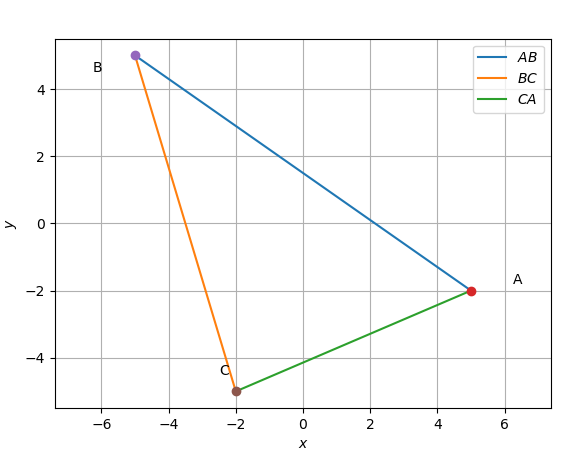
\includegraphics[width=\columnwidth]{/sdcard/Documents/fwc/moudle2/figs/ABCtriangle.png}
\caption{$\vec{A},\vec{B},\vec{C}$ plot}
\label{fig1:Triangle}
\end{figure}



\item The parameteric form of the equation  of $AB$ is 
		\begin{align}
			\vec{x}=\vec{A}+k\vec{m}
		\end{align}
		where
		\begin{align}
\vec{m}=\vec{B}-\vec{A}
		\end{align}
is the direction vector of $AB$.\\
Question 1.1.4 :Find the parametric equation of $AB$,$BC$,$CA$.\\
\solution
The parametric equation for AB is given by
\begin{align}
\vec{x} &= \vec{A} + k\vec{m}\\
\text{where, } \vec{m} &= \vec{B} -\vec{A}\\
&= \myvec{-10 \\7}
\end{align}
Hence we get,
\begin{align}
AB: \vec{x} = &\myvec{5\\-2} + k \myvec{-10\\7}
\end{align}
Similarly, 
\begin{align}
BC: \vec{x} = &\myvec{-5\\5} + k \myvec{3\\-10}\\
CA: \vec{x} = &\myvec{-2\\-5} + k \myvec{7\\-3}
\end{align}


\item The normal form of the equation of $AB$  is 
		\begin{align}
			\vec{n}^{\top}\brak{	\vec{x}-\vec{A}} = 0
		\end{align}
		where 
		\begin{align}
			\vec{n}^{\top}\vec{m}&=\vec{n}^{\top}\brak{\vec{B}-\vec{A}} = 0
			\\
			\text{or, } \vec{n}&=\myvec{0 & 1 \\ -1 & 0} \vec{m}
		\end{align}
  \begin{align}
\vec{n}^{\top}\myvec{\vec{x}-\vec{A}}=0
\end{align}
where
\begin{align}
\vec{n}^{\top}\vec{m}&=\vec{n}^{\top}\myvec{\vec{B}-\vec{A}}=0
\end{align}	
or,\begin{align}
\vec{n}&=\myvec{0 &1 \\-1 & 0}\vec{m}
\end{align}
Question 1.1.5:Find the normal form of the equations of $AB, BC$ and $CA$.\\
\solution:
       The normal equation for the side $AB$ is
\begin{align}
\vec{n}^{\top}\myvec{\vec{x}-\vec{A}}&=0\\
\implies
\vec{n}^{\top}\vec{x}&=\vec{n}^{\top}\vec{A}
\end{align}
Now our task is to find the $\vec{n}$ so that we can find $\vec{n}^{\top}$.
As given in the question 
\begin{align}
  \vec{n} &= \myvec{0 & 1\\
  -1 & 0}\vec{m}
\end{align}
Here $\vec{m} = \vec{B}- \vec{A}$ for side $\vec{AB}$
\begin{align}
\implies
\vec{m}&=\myvec{-5\\5} - \myvec{5\\-2}\\
&=\myvec{-10\\7}
\end{align}
Now as we have obtained vector $\vec{m}$.
we can use this to obtain vector $\vec{n}$
\begin{align}
\vec{n} &= \myvec{0 & 1\\
  -1 & 0}\myvec{-10\\7}
 = \myvec{7\\10}
\end{align}
The transpose of $\vec{n}$ is
\begin{align}
  \vec{n}^{\top}&=\myvec{7 & 10}
\end{align}
Hence the normal equation of side $AB$ is 
\begin{align}
    \myvec{7 & 10}\vec{x}&=\myvec{7 & 10}\myvec{5\\-2}\\
    \implies
    \myvec{7 & 10}\vec{x}&=15
\end{align}
\begin{figure}
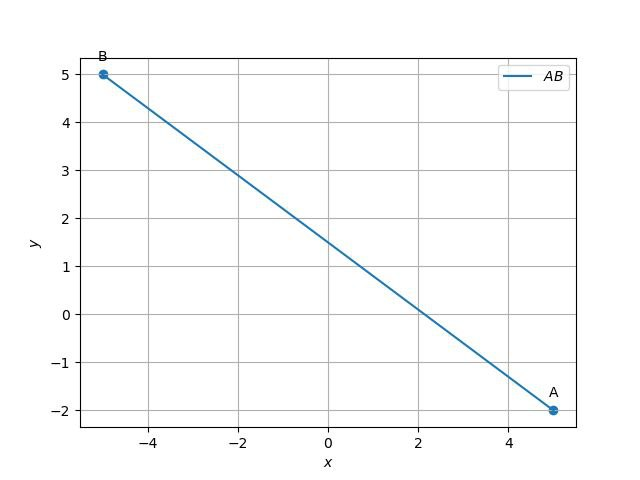
\includegraphics [width=\columnwidth]{/sdcard/Documents/fwc/moudle2/figs/ABline.png}
\caption{ The line $\vec{AB}$ plotted using python}
\label{fig: lineab}
\end{figure}


       The normal equation for the side $BC$ is
\begin{align}
\vec{n}^{\top}\myvec{\vec{x}-\vec{B}}&=0\\
\implies
\vec{n}^{\top}\vec{x}&=\vec{n}^{\top}\vec{B}
\end{align}
Now our task is to find the $\vec{n}$ so that we can find $\vec{n}^{\top}$.
As given in the question 
\begin{align}
  \vec{n} &= \myvec{0 & 1\\
  -1 & 0}\vec{m}
\end{align}
Here $\vec{m} = \vec{C}- \vec{B}$ for side $\vec{BC}$
\begin{align}
\implies
\vec{m}&=\myvec{-2\\-5} - \myvec{-5\\5}\\
&=\myvec{3\\-10}
\end{align}
Now as we have obtained vector $\vec{m}$.
we can use this to obtain vector $\vec{n}$
\begin{align}
\vec{n} &= \myvec{0 & 1\\
  -1 & 0}\myvec{3\\-10}
 = \myvec{-10\\-3}
\end{align}
The transpose of $\vec{n}$ is
\begin{align}
  \vec{n}^{\top}&=\myvec{10 & -3}
\end{align}
Hence the normal equation of side $BC$ is 
\begin{align}
    \myvec{10 & -3}\vec{x}&=\myvec{10 & -3}\myvec{-5\\5}\\
    \implies
    \myvec{10 & -3}\vec{x}&=-35
\end{align}
\begin{figure}
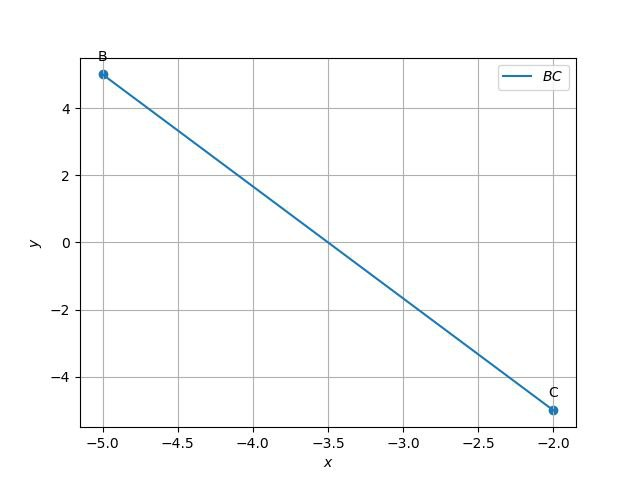
\includegraphics [width=\columnwidth]{/sdcard/Documents/fwc/moudle2/figs/BCline.png}
\caption{ The line $\vec{BC}$ plotted using python}
\label{fig: linebc}
\end{figure}



       The normal equation for the side $CA$ is
\begin{align}
\vec{n}^{\top}\myvec{\vec{x}-\vec{C}}&=0\\
\implies
\vec{n}^{\top}\vec{x}&=\vec{n}^{\top}\vec{C}
\end{align}
Now our task is to find the $\vec{n}$ so that we can find $\vec{n}^{\top}$.
As given in the question 
\begin{align}
  \vec{n} &= \myvec{0 & 1\\
  -1 & 0}\vec{m}
\end{align}
Here $\vec{m} = \vec{A}- \vec{C}$ for side $\vec{CA}$
\begin{align}
\implies
\vec{m}&=\myvec{5\\-2} - \myvec{-2\\-5}\\
&=\myvec{7\\3}
\end{align}
Now as we have obtained vector $\vec{m}$.
we can use this to obtain vector $\vec{n}$
\begin{align}
\vec{n} &= \myvec{0 & 1\\
  -1 & 0}\myvec{7\\3}
 = \myvec{3\\-7}
\end{align}
The transpose of $\vec{n}$ is
\begin{align}
  \vec{n}^{\top}&=\myvec{3 & -7}
\end{align}
Hence the normal equation of side $CA$ is 
\begin{align}
    \myvec{3 & -7}\vec{x}&=\myvec{3 & -7}\myvec{-2\\-5}\\
    \implies
    \myvec{3 & -7}\vec{x}&=29
\end{align}
\begin{figure}
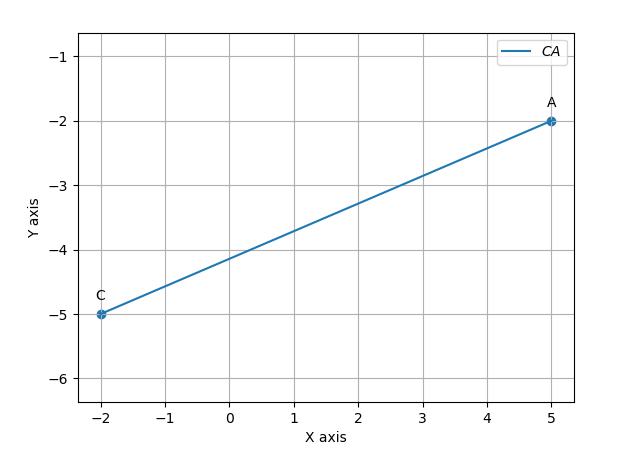
\includegraphics [width=\columnwidth]{/sdcard/Documents/fwc/moudle2/figs/ACline.png}
\caption{ The line $\vec{CA}$ plotted using python}
\label{fig: lineca}
\end{figure}


\item The area of $\triangle ABC$ is defined as
		\begin{align}
			\frac{1}{2}\norm{{\brak{\vec{A}-\vec{B}}\times {\vec{A}-\vec{C}}}}
		\end{align}
		where
		\begin{align}
			\vec{A}\times\vec{B} \triangleq \mydet{5 & -2 \\-5 & 5}
		\end{align}
Question 1.1.6:Find the area of $\triangle$ ABC.\\
\solution
Given,
\begin{align}
\vec{A} = \myvec{5\\-2};
\vec{B} = \myvec{-5\\5};
\vec{C} = \myvec{-2\\-5}\\
\vec{A}-\vec{B}=\myvec{5\\-2}-\myvec{-5\\5}&=\myvec{7\\-7}\\
\vec{A}-\vec{C}=\myvec{5\\-2}-\myvec{-2\\-5}&=\myvec{7\\3}\\
\therefore(\vec{A}-\vec{B})\times(\vec{A}-\vec{C}) &=\mydet{-7 & 7\\-7 & 3}\\&=70\\
\implies\frac{1}{2}\norm{(\vec{A}-\vec{B})\times(\vec{A}-\vec{C})}&=\frac{70}{2}=35
\end{align}


\item
Question 1.1.7:Find the angles $\vec{A},\vec{B},\vec{C}$, given that 
\begin{align}
	\cos{A} \triangleq \frac{(\vec{B}-\vec{A})\top(\vec{C}-\vec{A})}{\norm{\vec{B}-\vec{A}}\norm{\vec{C}-\vec{A}}}
\end{align}
\solution 
\\
From the given values of $\vec{A},\vec{B},\vec{C}$,\\
\begin{enumerate}

\item Finding the value of angle A
\begin{align}
	\vec{B}-\vec{A} &=\myvec{-10\\7}
\end{align}
and 
\begin{align}
	\vec{C}-\vec{A}&= \myvec{-7\\-3}
\end{align}
also calculating the values of norms
\begin{align}
	\norm{\vec{B}-\vec{A}} &= \sqrt{149} \\
	\norm{\vec{C}-\vec{A}} &= \sqrt{58} 
\end{align}
and by doing matrix multiplication we get,
\begin{align}
\begin{split}
	(\vec{B}-\vec{A})^{\top}(\vec{C}-\vec{A})&=\myvec{-10&7}\myvec{-7\\-3}\\
	&=49
\end{split}
\end{align}
so 
\begin{align}
	\cos{A}&= \frac{49}{\sqrt{149} \sqrt{58}}
	\implies A&=\cos^{-1}{ \frac{49}{\sqrt{149} \sqrt{58}}}
\end{align}




\item Finding the value of angle B
\begin{align}
	\vec{C}-\vec{B} &=\myvec{3\\-10}
\end{align}
and 
\begin{align}
	\vec{A}-\vec{B}&= \myvec{10\\-7}
\end{align}
also calculating the values of norms
\begin{align}
	\norm{\vec{C}-\vec{B}} &= \sqrt{109}\\
	\norm{\vec{A}-\vec{B}} &= \sqrt{149}
\end{align}
and by doing matrix multiplication we get,
\begin{align}
\begin{split}
	(\vec{C}-\vec{B})^{\top}(\vec{A}-\vec{B})&=\myvec{3&-10}\myvec{10\\-7}\\
	&= 100
\end{split}
\end{align}
so 
\begin{align}
	\cos{B}&= \frac{100}{\sqrt{109} \sqrt{149}}
	\implies B&=\cos^{-1}{ \frac{100}{\sqrt{109} \sqrt{149}}}
\end{align}



\item Finding the value of angle C
\begin{align}
	\vec{A}-\vec{C} &=\myvec{7\\3}
\end{align}
and 
\begin{align}
	\vec{B}-\vec{C}&= \myvec{-3\\10}
\end{align}
also calculating the values of norms
\begin{align}
	\norm{\vec{A}-\vec{C}} &= \sqrt{58}\\
	\norm{\vec{B}-\vec{C}} &= \sqrt{109}
\end{align}
and by doing matrix multiplication we get,
\begin{align}
\begin{split}
	(\vec{A}-\vec{C})^{\top}(\vec{B}-\vec{C})&=\myvec{7&3}\myvec{-3\\10}\\
	&=9
\end{split}
\end{align}
so 
\begin{align}
	\cos{C}&= \frac{9}{\sqrt{58} \sqrt{109}}
	\implies C&=\cos^{-1}{ \frac{9}{\sqrt{58} \sqrt{109}}}
\end{align}
\end{enumerate}
\end{enumerate}
%\section{Median}
%\input{subsec/median}
%\section{Altitude}
%\section{Perpendicular Bisector}
%\section{Angle Bisector}
\end{document} 
